\vspace{0.5cm}
\section{Table de symboles}

\vspace{0.5cm}
Avant de rentrer dans le vif du sujet, il est important de spécifier comment chaque identifiant est géré.

\vspace{0.5cm}
Deux choses nous ont poussés à implémenter un système de tables de symboles :
\begin{itemize}
\item Dans un premier temps, les variables étant stockées dans la pile, on va avoir besoin de connaître leur position pour pouvoir y accéder. A chaque symbole sera donc associé un offset.
\item Ensuite, lorsque l'on a plusieurs blocs d'instructions, les variables ne sont pas forcément visibles dans chaque bloc. Il va donc être nécessaire d'établir un arbre de tables de symboles, où chaque n\oe{}ud est propre à un bloc, et n'a de visibilité que dans sa propre liste de symboles et dans celles de la branche qui le relie à la table racine.
\end{itemize}


\subsection*{Structures}

\vspace{0.5cm}
Pour gérer ce système, nous utilisons trois structures en terme de programmation C.

\vspace{0.5cm}
Tout d'abord, une structure pour décrire chaque n\oe{}ud de l'arbre, c'est à dire chaque table. 

\begin{verbatim}
struct symbolTableTreeNode
{
  struct symbolTableTreeNodeList* sons;
  struct symbolTableTreeNode* father;
  struct symbolTableIdentifierList* identifierList;
  char* functionName;
  struct string* code;
  int currentOffset;
  int parameterSize;
};
\end{verbatim} 

Elle est composée d'un champ father, et d'un champ sons pour permettre la navigation dans l'arbre. 

Le champ identifierList correspond aux symboles en eux-même. Il s'agit d'une liste. 
functionName et parameterSize sont des champs qui décrivent la fonction, c'est à dire son nom, et la taille de ses paramètres. Si le bloc d'instructions ne correspond pas à une fonction, ces champs restent nuls.

currentOffset correspond au FramePointer et permet de définir le début de la fonction dans la pile, et donc sa visibilité.

Le champ code est relativement important pour comprendre comment nous gérons la génération du code. Chaque table correspond à un bloc d'instructions. Parfois, nous le verrons plus tard dans ce rapport, il est nécessaire de connaître l'ensemble des instructions avant d'écrire le code. Dans un premier temps, les instructions générées sont donc stockées dans le champ code. Cela nous permet de les imprimer seulement au moment où toutes les informations nécessaires sont connues.


\vspace{0.5cm}
La structure qui suit décrit un étage de l'arbre. Il s'agit d'une liste de tables des symboles situés à une même distance de la racine.

\begin{verbatim} 
 struct symbolTableTreeNodeList
{
  struct symbolTableTreeNodeList* next;
  struct symbolTableTreeNode* data;
};
\end{verbatim} 

\vspace{0.5cm}
Enfin, voici la liste des symboles en elle-même.

\begin{verbatim}
struct symbolTableIdentifierList
{
  struct symbolTableIdentifierList* next;
  char* name;
  int type;
  int offset;
  int size;
  int nbArrayDimension;
  int dimensionSizes[256];
};
\end{verbatim} 
 
Elle contient bien évidemment un pointeur vers l'élément suivant.

Elle contient de plus toutes les informations concernant un symbole, c'est à dire son nom, son type, son offset (sa position dans la pile), et sa taille.

Dans le cas d'un tableau, elle possède aussi sa dimension, et la taille de chacun des vecteurs qui le composent.

\vspace{0.5cm}
\newpage
Graphiquement, nous avons donc le système qui suit : 

\begin{figure}[h!]
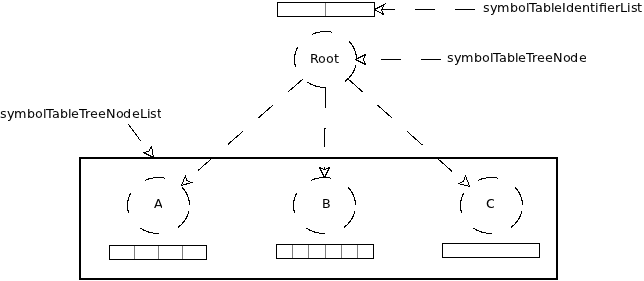
\includegraphics[scale=0.5]{arbresym.png}
\end{figure}

Ici, Root a pour father NULL, et pour sons A, B et C.

Les tables B et C ont toutes pour père Root, et pas de fils.
A a pour père father, et pour fils D. Cette dernière a donc pour père A, et pas de fils.

Root a deux éléments dans sa table des symboles, A quatre, B six, C un seul et D, deux.